\chapter{Конструкторский раздел}


\section{Углы Эйлера}
\hspace{0.6cm}Углы Эйлера определяют три поворота системы, которые позволяют привести любое положение системы к текущему. Обозначим начальную систему координат как (x, y, z) , конечную как (X,Y,Z). Пересечение координатных плоскостей xy и XY называется линией узлов N.
\begin{itemize}
	\item Угол a между осью x и линией узлов — угол прецессии.
	\item Угол b между осями z и Z — угол нутации.
	\item Угол y между линией узлов и осью  X— угол собственного вращения.
\end{itemize}

\hspace{0.6cm}Повороты системы на эти углы называются прецессия, нутация и поворот на собственный угол (вращение). Такие повороты некоммутативны и конечное положение системы зависит от порядка, в котором совершаются повороты. В случае углов Эйлера производится серия из трёх поворотов:
\begin{enumerate}
	\item На угол a вокруг оси z. При этом ось x переходит в N.
	\item На угол b вокруг оси N. При этом ось z переходит в Z.
	\item 	На угол y вокруг оси Z. При этом ось N переходит в X.
\end{enumerate}
Иногда такую последовательность называют 3,1,3 (или Z,X,Z), но такое обозначение может приводить к двусмыслице.


\section{Структура проверок положения точек}
\hspace{0.6cm}Входные данные в программу представляют собой 42 точки в трехмерном пространстве. Из 42 точек, 21 определяет одну кисть.

\hspace{0.6cm}Проверка кисти на правильность осуществляется с помощью группы проверок отдельных пальцев, а также точек расположенных непосредственно на ладони. Для реализации проверок лучше использовать язык программирования Prolog, поскольку это мощный инструмент именно для работы с логическими конструкциями.

\hspace{0.6cm}Для удобства представления входных данных их можно разделить на структуры. 
\begin{figure}[ht!]
	\centering
	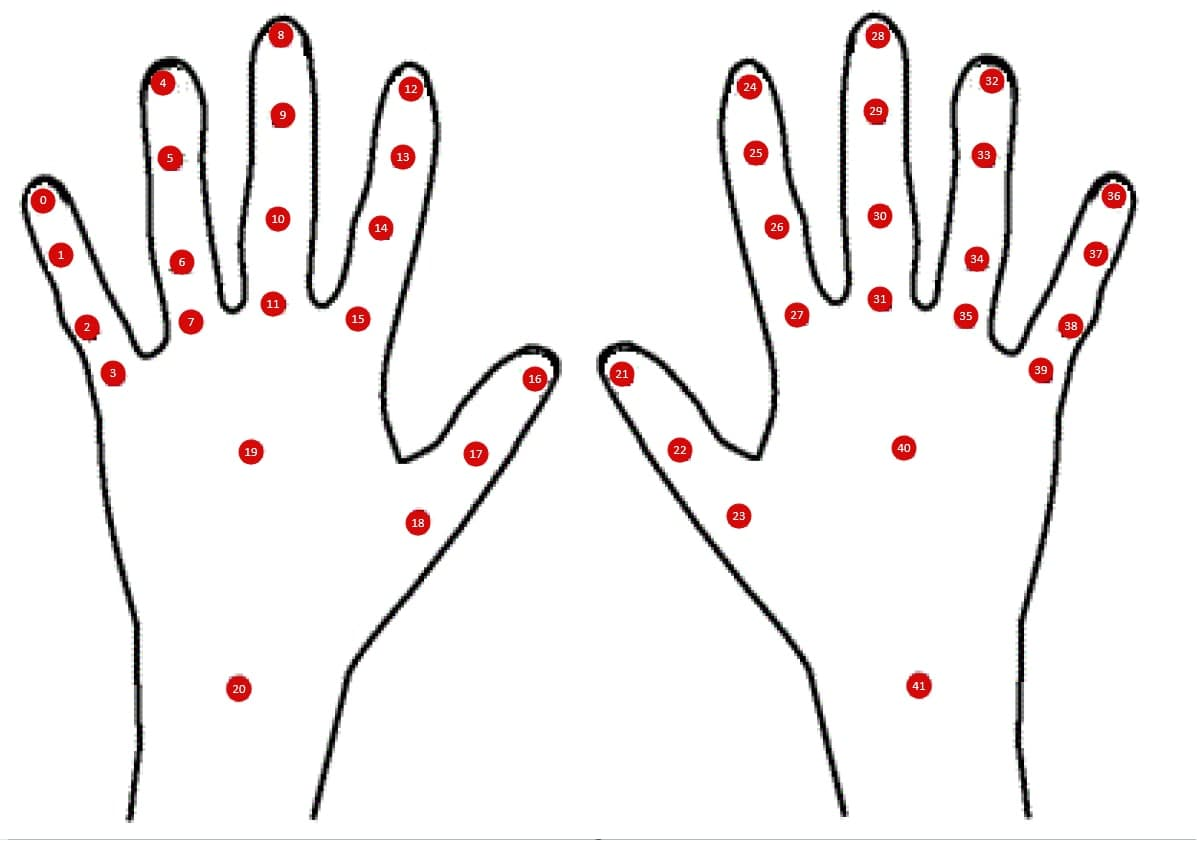
\includegraphics[scale=0.4]{Kist.jpg}
	\caption{Нумерация точек на кисти}
	\label{fig:hands}
\end{figure}
\hspace{0.6cm}Возьмем точки 0, 1, 2, 3. Вместе они составляют мизинец на руке. В соотвествии с этим можно создать структуру мизинца. Схожим образом можно объединить оставшиеся точки в безымянный, средний, указательный и большой пальцы. Остануться только точки 19, 20 на левой руке и 40, 41 на правой. Эти точки являются ключевыми для своих кистей соотвественно.
\hspace{0.6cm}Далее полученные структуры пальцев мы можем обьединить в структуру руки. Каждая рука будет состоять из пальцев и оставшимся двум точкам соответсвенно для левой и правой кисти. 
\hspace{0.6cm}Данные преобразования необходимо провести для упрощения понимания структуры кода при его чтении, а также облегчения работы при написании процедур проверок.
\hspace{0.6cm}Сами проверки в своей основе опираются на проверку углов между определенными точками в пальце.  

\section{Визуализация руки}

